\section{Kapitel 2} 
\subsection{mängder}
    \label{mängder}
    \textbf{\cite{mängder}} Med en mängd menar vi en väldefinerad samling av olika objekt som vi kallar element. Att en mängd är väldefineread innebär att man kan avgöra om ett godtyckligt objekt är element i mängden eller ej.
    \par Vi betecknar oftast mängder med stora bokstäver: $A,B,C,X,Y,Z,...$, medan element i mängderna betecknas med små bokstäver: $a,b,c,x,y,z,...$. Om $x$ är ett element i en mängd $M$, skriver vi $x \in M$, vilket utläses "$x$ \textbf{tillhör} $M$", annars skriver vi $x \notin M$, som utläses "$x$ \textbf{tillhör inte} $M$".
    \par En mängd $M$ med ändligt antal element kan beskrivas genom att man räknar upp mängdens element inom \textbf{mängdklamrar}, d.v.s. symbolerna \textbf{\{} och \textbf{\}}, men oftare beskriver man en mänd genom att ange de egenskaper som utmärker $M$:s element.
        \paragraph{Exempel} Mängden $M$ består av talen -3, -1, 1 och 3. Vi kan beskriva $M$ genom att räkna upp elementen: 
            \begin{center}
                $M = \{-3, -1, 1, 3\}.$
            \end{center}
        \paragraph{Exempel} Vi kan också beskriva $M$ genom att räkna upp de egenskaper som utmärker $M$:s element:
            \begin{center}
                $M = \{ x:x$ är ett udda heltal och $-3 \leqslant x \leqslant 3 \}.$
            \end{center}
\subsection{delmängder}
    \label{delmängder}
    Låt $A$ och $B$ vara två mängder[\ref{mängder}]. Vi säger att $A$ är en \textbf{delmängd} till $B$ om varje element i $A$ också är ett element i $B$. Denna relation betecknas
        \begin{center}
            $A \subseteq B.$
        \end{center}
    Om det dessutom finns minst ett element i $B$ som inte tillhör $A$, säger vi att $A$ är en \textbf{äkta delmängd} till $B$ och skriver
        \begin{center}
            $A \subset B.$
        \end{center}
\subsection{venndiagram}
    \label{venndiagram}
    \cite{venndiagram} I många sammanhang är det naturligt att tänka sig alla förekommande mängder som delmängder till något fixerat \textbf{universum} eller en \textbf{grundmängd} som betecknas $\mathcal{U}$ illustreras med en rektangel och alla delmängder till $\mathcal{U}$ markeras med cirklar inom denna rektangel.
        \begin{center}
            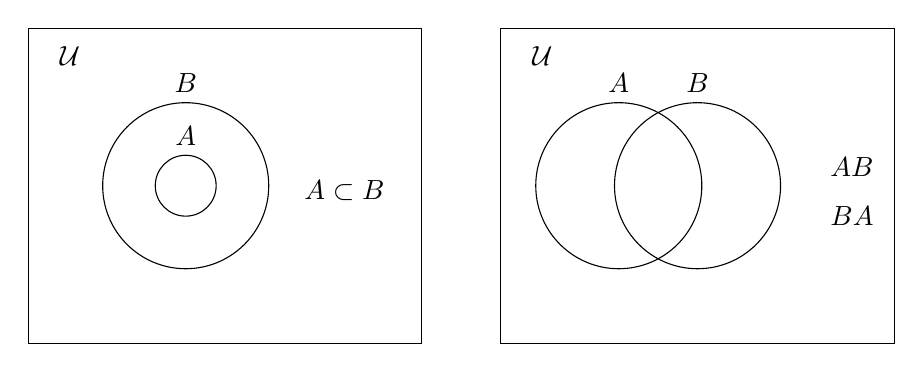
\begin{tikzpicture}
                % universum 1 & 2.
                \draw (0,0) rectangle (5,4) 
                    node[below = 10pt, left = 120pt] {$\mathcal{U}$}
                    node[below = 58.5pt, left = 10pt] {$A \subset B$};
                \draw (6,0) rectangle (11,4) 
                    node[below = 10pt, left = 120pt] {$\mathcal{U}$}
                    node[below = 50pt, left = 4pt] {$A \nsubseteq B$}
                    node[below = 68pt, left = 4pt] {$B \nsubseteq A$};
                % mängder till universum 1.
                \draw (2,2) circle (11pt) node[above = 11pt] {$A$};
                \draw (2,2) circle (30pt) node[above = 30pt] {$B$};
                % mängder till universum 2.
                \draw (7.5,2) circle (30pt) node[above = 30pt] {$A$};
                \draw (8.5,2) circle (30pt) node[above = 30pt] {$B$};
            \end{tikzpicture}
        \end{center}
    